\documentclass{report_template_oxford}

\usepackage{float}

\title{Laser Tag using a Multiagent Drone System}
\subtitle{Report for the system and software design of a multiagent drone system to play Laser Tag}
\author{Shing Hei Rickie Chan, Thomas August, Rishabh Luthra, Richard Usherwood}
\date{March 2026}

\begin{document}
\maketitle
\pagenumbering{roman}
\newpage

% Abstract
% - Concise summary of report
% - Naming of essential outcomes
% - As short as possible while providing key points
% - Less than 1 page
\addcontentsline{toc}{section}{Abstract}
\fancyhead[C]{Student author of section}
\section*{Abstract}
\newpage

\fancyhead[C]{}
\tableofcontents
\newpage

\addcontentsline{toc}{section}{List of Figures}
\listoffigures
\newpage

\addcontentsline{toc}{section}{List of Tables}
\listoftables
\newpage

\addcontentsline{toc}{section}{Glossary}
\newacronym{3yp}{3YP}{Third-Year Project}
\newacronym{fov}{FoV}{Field of View}
\printglossaries
\newpage

\pagenumbering{arabic}

% Introduction
% - Provide background and motivation
% - Provide boundaries and goals to the project
% - Give a short overview of report structure
\section{Introduction}
\fancyhead[C]{Student2 author of section}
\subsection{An awesome Acronym}
You can use acronyms for your \gls{3yp} exactly as I did here.
You can define them in the header of this file and they will appear in the glossary section. 
\newpage

\section{Literature Review}
\newpage

\section{System Architecture and Integration} % Everyone
\newpage

\section{Hardware} % Rickie
\subsection{CAD Design}

\section{Sensor Processing} % Tommy, Rishabh
\subsection{Player detection} % Rishabh
\subsection{Drone pose tracking} % Tommy


\section{High Level Control} % Ritchie
\newpage

\section{Mid Level Control} % Tommy, Rishabh
\subsection{Visual Perception and Player Tracking} % Rishabh
\subsubsection{Subsystem Context}
The fundamental objective of the autonomous multiagent system is to actively compete against human players in a dynamic laser environment. To play the game effectively, the drones require a reliable way to identify and track opponents whilst navigating through the maze environment. While pathfinding algorithms can navigate the fixed geometry of a maze, human players represent highly dynamic variables. Therefore, a real-time perception system is required to continuously locate the targets, maintain visual lock, and output kinematic commands to the drone's flight controller and gimbal.

This section details the design and implementation of this perception system. To achieve these operational requirements, the subsystem is engineered around three core objectives:
\begin{itemize}
    \item Reliably distinguishing a human player from background obstacles and other drones to ensure that the system locks onto the correct target.
    \item Calculating the target's 3D Cartesian coordinates relative to the drone's local frame.
    \item Maintaining a continuous state estimate of the target's trajectory to handle temporary line-of-sight occlusions caused by walls and obstacles.
\end{itemize}

\subsubsection{Hardware Selection} % (Rishabh - can be moved somewhere else, just put it here to make sure it's covered)
In order to transition from the objectives to the physical implementation, we require a sensor payload that can provide high-fidelity data without compromising flight performance or game mechanics. 

Quadcopters are inherently underactuated mechanical systems [ref]; to achieve horizontal translation, the drone must pitch ($\theta$) or roll ($\phi$) in the direction of travel. If the visual sensor is rigidly mounted to the chassis, any forward acceleration pitches the sensor towards the floor, which may force the target out of the \gls{fov}. In order to resolve this, the sensor payload must be mounted to a 3-axis active gimbal. The gimbal acts as a kinematic decoupler, executing rotation transformations to maintain the camera frame at a fixed angle relative to the horizon, regardless of the drone's orientation.

To achieve 3D spatial localisation of the target, the specific imaging hardware must be selected. This choice is governed by two constraints: SWaP-C (Size, Weight, Power, and Cost) for flight agility, as well as how well the imaging hardware integrates into the environment. A further requirement from the imaging hardware is its ability to extract the depth of the target. 




%As a result, this section aims to justify the selection of the Raspberry Pi AI Camera as well as the integration of a 3-axis gimbal mounted underneath the drone.


\newpage
\subsection{Trajectory tracking} % Tommy
\subsection{Searching} % Maybe Tommy
\subsection{Hiding} % Not implemented but talk about it

\section{Low Level Control} % Tommy, Rishabh
\subsection{Conversion Matrix}
\newpage


\section{App} % Ritchie
\subsection{Motivation}
From fast-food restaurants to road cycling, apps are everywhere. Their purpose can be separated into two categories: Engagement and Functionality.

They encourage user-engagement by allowing users to track their progress through points and achievements, customise their profiles, and connect with friends. For example, popular birdwatching app "Birda" is used by users to log bird sightings. It rewards users with achievement badges when they complete objectives (for example, seeing ten different species), and integrates monthly challenges. It also connects birdwatchers through the "community" feature, allowing users to view their friends' activity and sightings by strangers in their area. 

Companion apps also serve a functional purpose. Since (almost) everyone in the UK owns and uses a smartphone, they can be directly implemented into the experience. For example, popular budget UK pub chain JD Wetherspoon uses a companion app to allow patrons to order drinks and food directly to their table, without requiring them to break conversation and queue at a busy bar. 
\subsection{Implementation with existing game}
When opened for the first time, the app prompts the user to create an account with a username and password. When completed, the app the first of five screens that are navigated using a bottom panel: the "Profile" screen, the "Leaderboard" screen, the "Achievements and Challenges" screen, the "Community" screen, and the "Play in Person" screen . The first four screens are engagement-based, and the fifth is functionality-based.
\subsubsection{Engagement}
The "Profile" screen displays the player's details (Player ID, name etc.), the score details (number of games played, number of kills and deaths, total score), and the player's social details (friends, friend requests). It also displays an optional profile picture, which is displayed to other players when viewing your profile in the leaderboard/community screens. The profile picture fosters the "community" feel of the app, and reduces confusion between multiple players with the same name.

The "Leaderboard" screen displays a list of players in order of their total score. The app user can toggle between viewing a global leaderboard and a leaderboard of only their friends.

The "Achievements and Challenges" screen displays all achievements (lifetime goals, for example "play ten games", "kill fifteen drones in one game", "be the last player alive in a death match" etc.), and monthly challenges (smaller achievements that reset and change every month). The inclusion of lifetime achievements allows for a long-term feeling of improvement, while the monthly challenges allow new players to compete with their more experienced friends.

The "Community" screen toggles between displaying details of recent games played by the app user's friends, and displaying details of all recent games played. It also allows users to search for other players by name, or by Player ID, and to send each other friend requests. This allows players to track each other's progress, and allows players to feel connected to friends they may have made through playing the game in person.
\subsubsection{Functionality}
The "Play in Person" screen prompts the player to scan the QR codes on the top of the laser gun and the helmet they are given when playing in-person. This allows the server to attribute the correct number of kills and deaths (infra-red strikes on drones, encoded with ID of the gun, and infra-red strikes on helmet detector, communicated with server) to the correct player, making for a seamless user experience.
\subsection{Technical Details}

\section{Commercialisation, Safety and Project Management} % Mostly Ritchie
\subsection{Risk Assessment}
\begin{figure}[H]
    \centering
    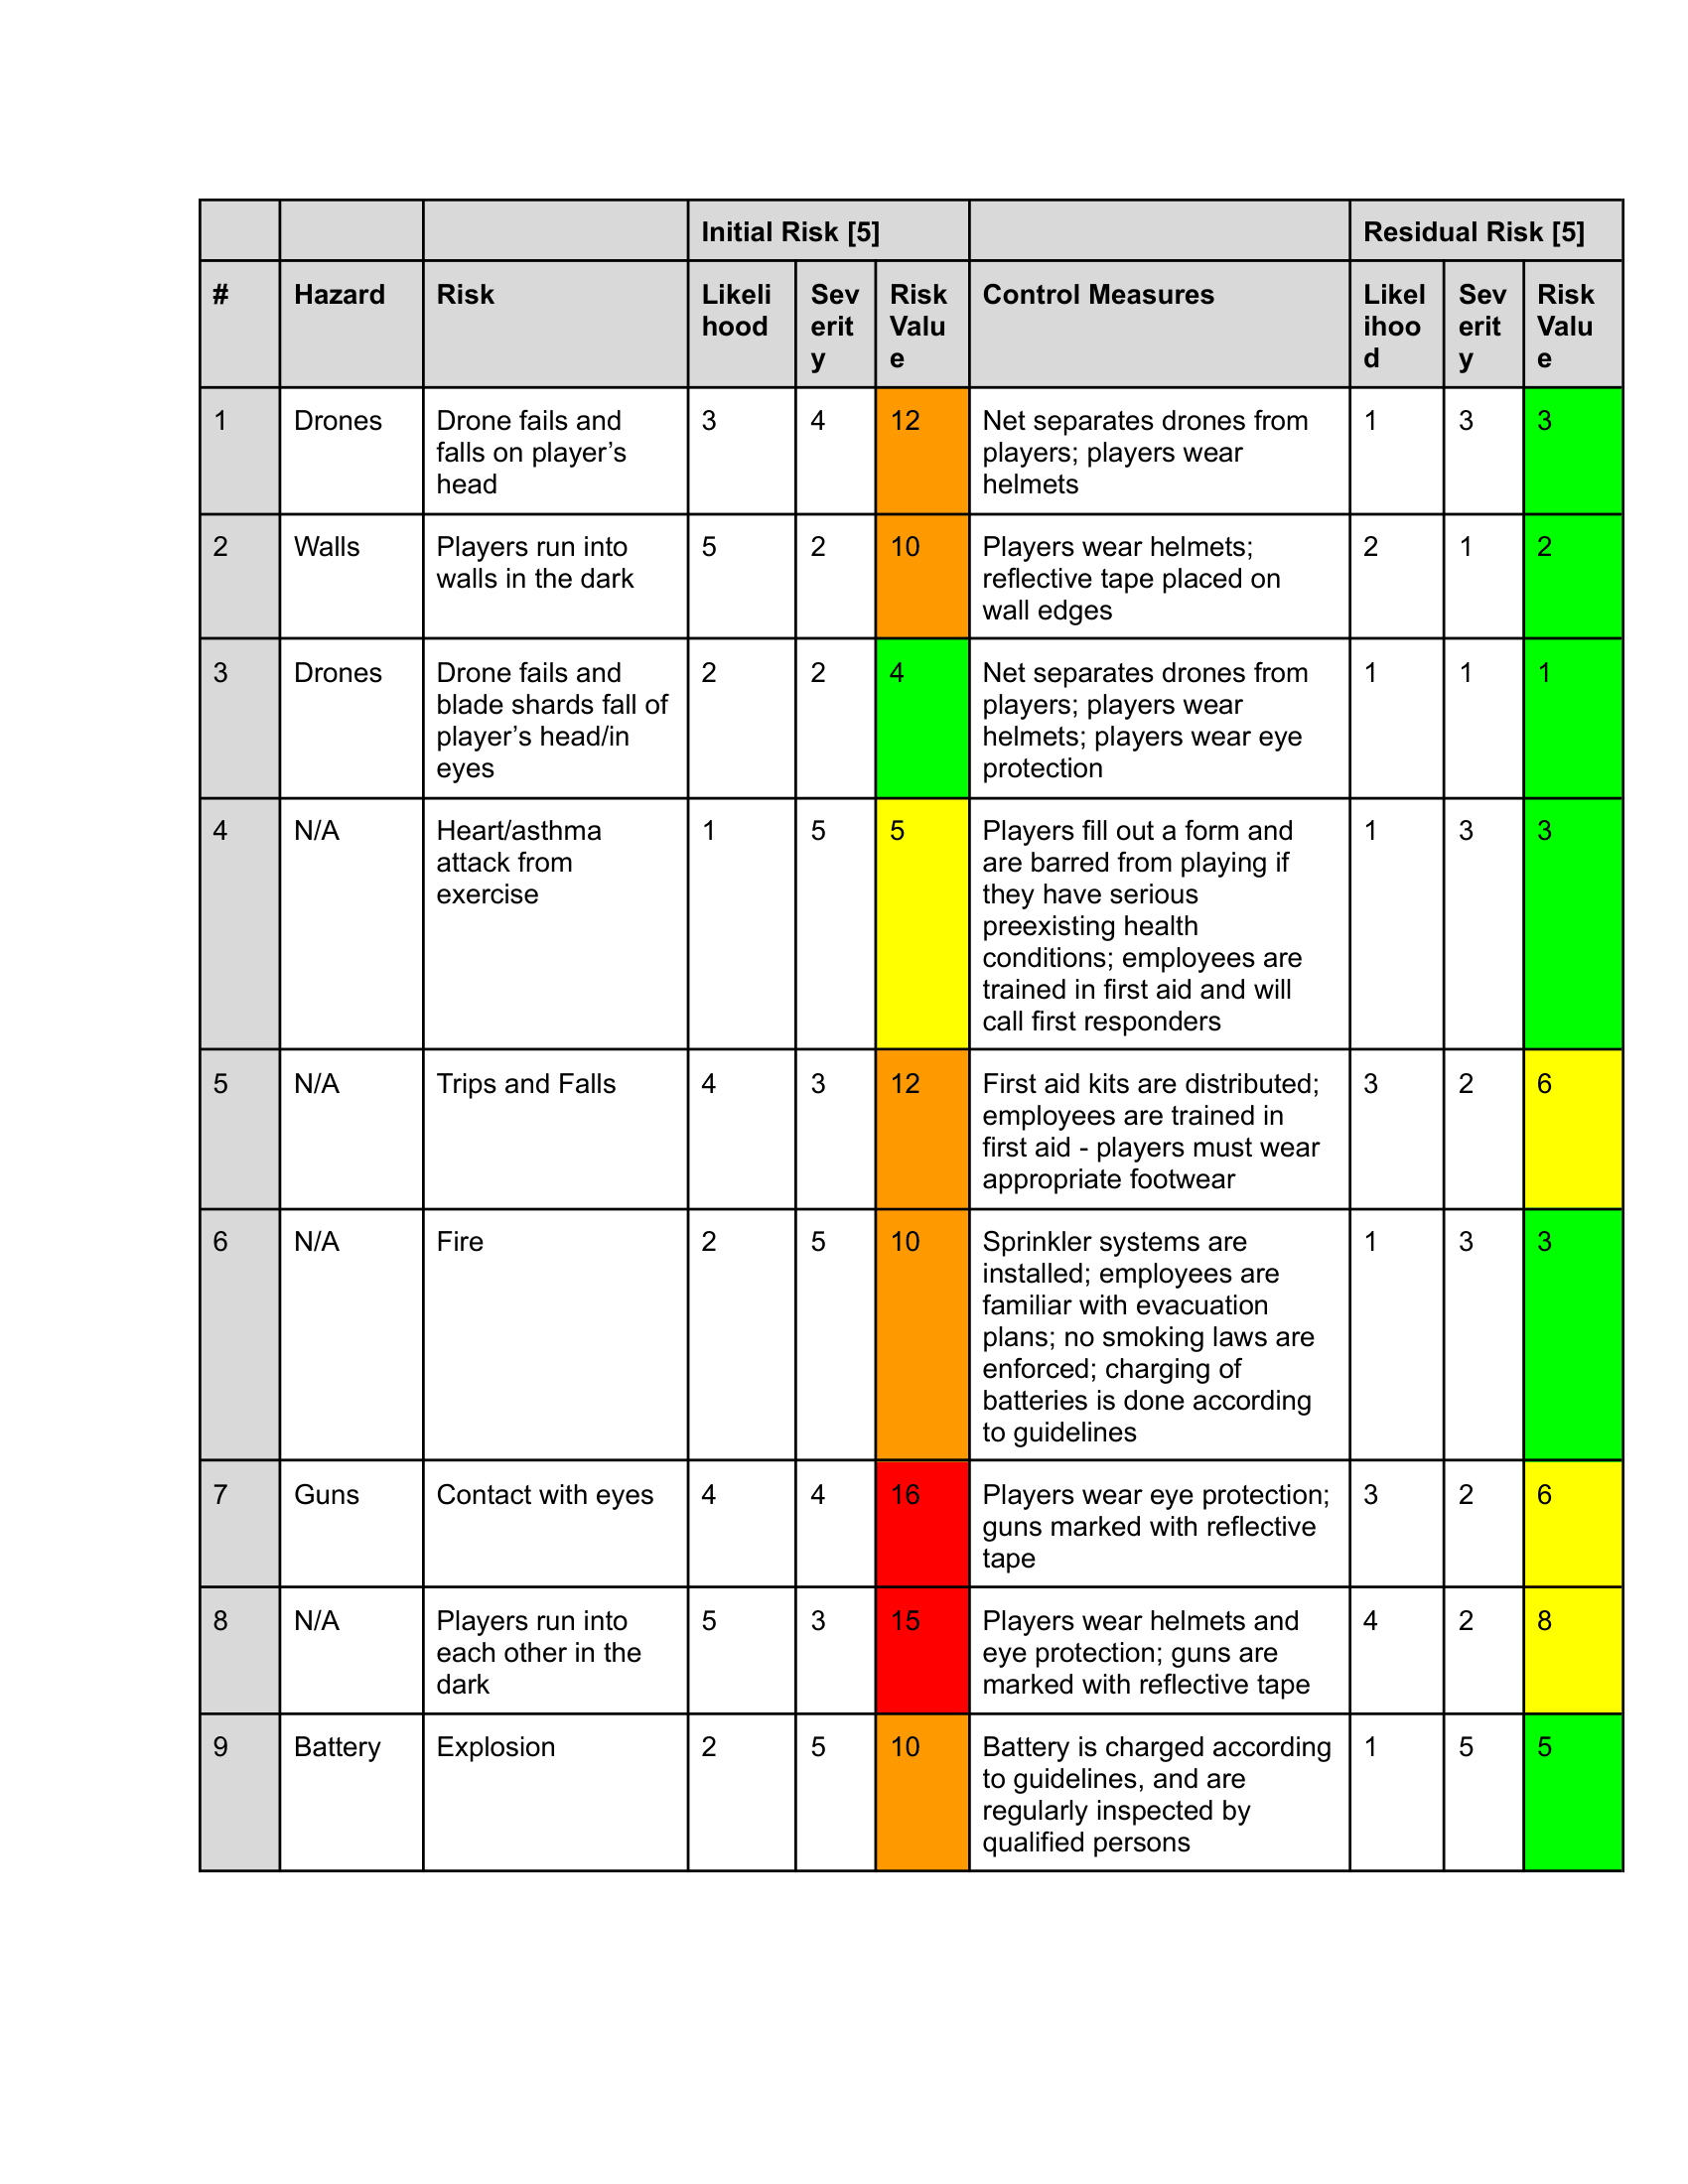
\includegraphics[width=1\linewidth]{figs/risk-assessment}
    \caption{Quantitative Risk Assessment.}
    \label{fig:risk-assessment}
\end{figure}

A quantitative risk assessment has been completed, and is shown in figure \ref{fig:risk-assessment}. As shown, the most significant initial risks were the the contact between guns and players' eyes, and players running into each other. After the necessary control measures, they are still most significant residual risks, along with trips and falls. This demonstrates that there is not an undue risk associated with playing the game, since trips and falls, player-on-player collision and impact with instruments used for playing (such as laser-guns, squash raquets etc.) are risks associated with traditional laser-tag, as well as many common sports. 
\subsection{Financing}
\subsection{Wake up the audience who've fallen asleep}
\newpage


% Appendix
% Essential content that interrupts the flow of the document can be placed here, e.g. technical drawings, detailed lists of equations used, etc.
\addcontentsline{toc}{section}{Appendix}
\section*{Appendix}
\newpage

\printbibliography{biblio}
\newpage


\end{document}
